Para a realização deste trabalho prático foi criado um ambiente com várias máquinas virtuais na mesma \ac{LAN}, utilizando o virtualizador VMWare.

\section{Endereçamento}

Administração:

\begin{table}[h]
\begin{center}
\begin{tabular}{||c c||} 
 \hline
 Nome & IP\\ [0.5ex] 
 \hline\hline
 Servidor DD1 & 192.168.1.129\\ 
 \hline
 Servidor DD2 & 192.168.1.130\\
 \hline
 Servidor DD3 & 192.168.1.131\\
 \hline
 VM & 192.168.1.128\\
 \hline
 CT & 192.168.1.140\\
 \hline
\end{tabular}
\caption{Tabela endereçamento \ac{IP}}
\end{center}
\end{table}

Rede do Cluster:

\begin{table}[h]
\begin{center}
\begin{tabular}{||c c||} 
 \hline
 Nome & IP\\ [0.5ex] 
 \hline\hline
 Servidor DD1 & 10.10.10.129\\ 
 \hline
 Servidor DD2 & 10.10.10.130\\
 \hline
 Servidor DD3 & 10.10.10.131\\
 \hline
\end{tabular}
\caption{Tabela endereçamento \ac{IP} do Cluster}
\end{center}
\end{table}

\section{Ambiente Proxmox}
\begin{figure}[H]
\center
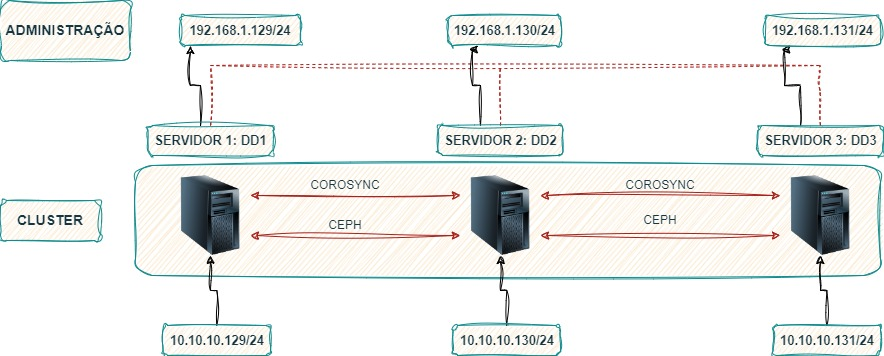
\includegraphics[width=15cm]{arquitetura.jpg}
\caption{Ambiente Proxmox}
\end{figure}

\section{Arquitetura dos Servidores}
\begin{itemize}
    \item CPU: 2;
    \item RAM: 4GB;
    \item Placa de Rede: 2;
    \item Disco: 120GB;
\end{itemize}

\begin{figure}[H]
\center
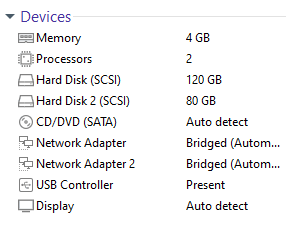
\includegraphics[width=15cm]{devices.png}
\caption{Devices}
\end{figure}
